% ════════════════════════════════════════════
% 4. 数据清洗与整理
% ════════════════════════════════════════════
\section{数据清洗与整理}

\subsection{缺失、异常与一致性}

全表逐列核查的结果见表\ref{tab:check}：只有 $X_7$ 缺失 1 条（第 499 行，占 0.2\%），其余字段完整，完全重复行 0 条。$X_7$ 为二元变量且自然帖占 72.2\%，按众数填补为 0 并保留填补标记；同时以删除该行的样本重估同一模型，核心系数差异小于 0.01，说明填补方式不影响结论。$Y_1$ 存在 1 条 1,110,282 次的极端记录，核对后确认为真实的病毒式传播而非录入错误，保留不动，由 $\log(1+Y_1)$ 变换压缩其影响。取值域检查全部通过：$X_7\in\{0,1\}$、$X_2$ 四类与文档一致、$X_3\in\{1,2,3\}$、$X_4\in\{1,\dots,12\}$、$X_5\in\{1,\dots,7\}$、$X_6$ 落在 0--23 内但样本中 0 时与 21 时没有帖子。

{\small
\begin{longtable}{>{\centering\arraybackslash}p{0.180\textwidth}>{\centering\arraybackslash}p{0.300\textwidth}>{\centering\arraybackslash}p{0.260\textwidth}>{\centering\arraybackslash}p{0.240\textwidth}}
  \caption{缺失、异常与一致性检查}
  \label{tab:check} \\
  \toprule
  检查项 & 实际结果 & 判断 & 处理 \\
  \midrule
  \endfirsthead
  \caption{缺失、异常与一致性检查（续）} \\
  \toprule
  检查项 & 实际结果 & 判断 & 处理 \\
  \midrule
  \endhead
  \bottomrule
  \endfoot
  X1 取值范围 & 81,370–139,441 & 在文档 81,370–139,441 内 & 保留 \\
  X2 取值集合 & Link、Photo、Status、Video & 4 类，与文档一致 & 转为名义变量 \\
  X3 取值集合 & 1、2、3 & 1/2/3，与文档一致 & 转为名义变量 \\
  X4 取值范围 & 1–12 & 1–12，无越界 & 保留并编码 \\
  X5 取值范围 & 1–7 & 1–7，无越界 & 保留并编码 \\
  X6 取值范围 & 1–23 & 0–23 内；样本 1–23，0 与 21 时无帖子 & 按分布合并为 3 组 \\
  X7 取值集合 & 0/1（缺失 1 条） & 二元变量；第 499 行缺失 & 众数填补 0，另做删除敏感性 \\
  Y1 取值范围 & 570–1,110,282 & 全部为正，与文档一致 & log1p 变换 \\
  完全重复行 & 0 条 & 无重复帖子 & 无需去重 \\
  异常值 & Y1 存在 1 条 1,110,282 的极端曝光 & 属真实病毒式传播，不是录入错误 & 保留，log 变换压缩 \\
  X7 填补 & 众数 0，共 1 条 & 填补后无缺失 & 保留填补标记 \\
\end{longtable}
}


\subsection{编码与变换}

编码方案见表\ref{tab:encode}，原则是让每个系数都有明确参照：名义变量做独热编码并指定参照类（$X_2$ 以 Photo、$X_3$ 以主题 1 为基线），周期变量同样按哑变量处理，二元变量保持 0/1，$X_1$ 取对数压缩量级，$Y_1$ 取 $\log(1+Y_1)$。24 小时的发布时段若逐小时生成哑变量会产生 22 个稀疏单元，因此按样本分布合并为凌晨（0--5 时）、上午（6--11 时）、下午晚间（12--23 时）三组，以样本量最大的上午为基线。

{\small
\begin{longtable}{>{\centering\arraybackslash}p{0.070\textwidth}>{\centering\arraybackslash}p{0.150\textwidth}>{\centering\arraybackslash}p{0.240\textwidth}>{\centering\arraybackslash}p{0.160\textwidth}>{\centering\arraybackslash}p{0.360\textwidth}}
  \caption{变量编码与变换方案}
  \label{tab:encode} \\
  \toprule
  变量 & 识别类型 & 编码/变换 & 基线/参照 & 解释 \\
  \midrule
  \endfirsthead
  \caption{变量编码与变换方案（续）} \\
  \toprule
  变量 & 识别类型 & 编码/变换 & 基线/参照 & 解释 \\
  \midrule
  \endhead
  \bottomrule
  \endfoot
  X1 & 连续 & log(X1) & — & 粉丝规模弹性；避免量级差异 \\
  X2 & 名义（4 类） & 独热编码，3 个哑变量 & Photo & 比 Photo 的相对曝光差异 \\
  X3 & 名义（3 类） & 独热编码，2 个哑变量 & 1 & 比主题 1 的相对曝光差异 \\
  X4 & 有序/周期（12） & 独热编码，11 个哑变量 & 1 月 & 控制季节性与时间趋势 \\
  X5 & 有序/周期（7） & 独热编码，6 个哑变量 & 周一 & 控制星期效应 \\
  X6 & 有序/周期（24） & 按分布合并为 3 组，2 个哑变量 & 上午（6–11 时） & 凌晨 0–5、上午 6–11、下午晚间 12–23；避免稀疏单元 \\
  X7 & 二元 & 0/1 数值 & 0（自然） & 付费的额外曝光 \\
  Y1 & 连续计数 & log1p(Y1) & — & 压缩重尾，系数近似百分比效应 \\
\end{longtable}
}


类别不平衡的实际情况见图\ref{fig:cat}：Photo 有 426 条（85.2\%），Status 45 条、Link 22 条、Video 仅 7 条（1.4\%）；付费占比在类型间差异明显，Video 组 7 条中有 4 条付费（57.1\%），Photo 组为 27.9\%。付费标记与缺失处置的结果一并画在左下角，缺失的 1 条在图中以斜纹柱标注。样本量过小的类别不删除——它们是回答“视频帖是否更有效”的唯一证据，但在解释时必须标注区间宽度。

\begin{figure}[htbp]
  \centering
  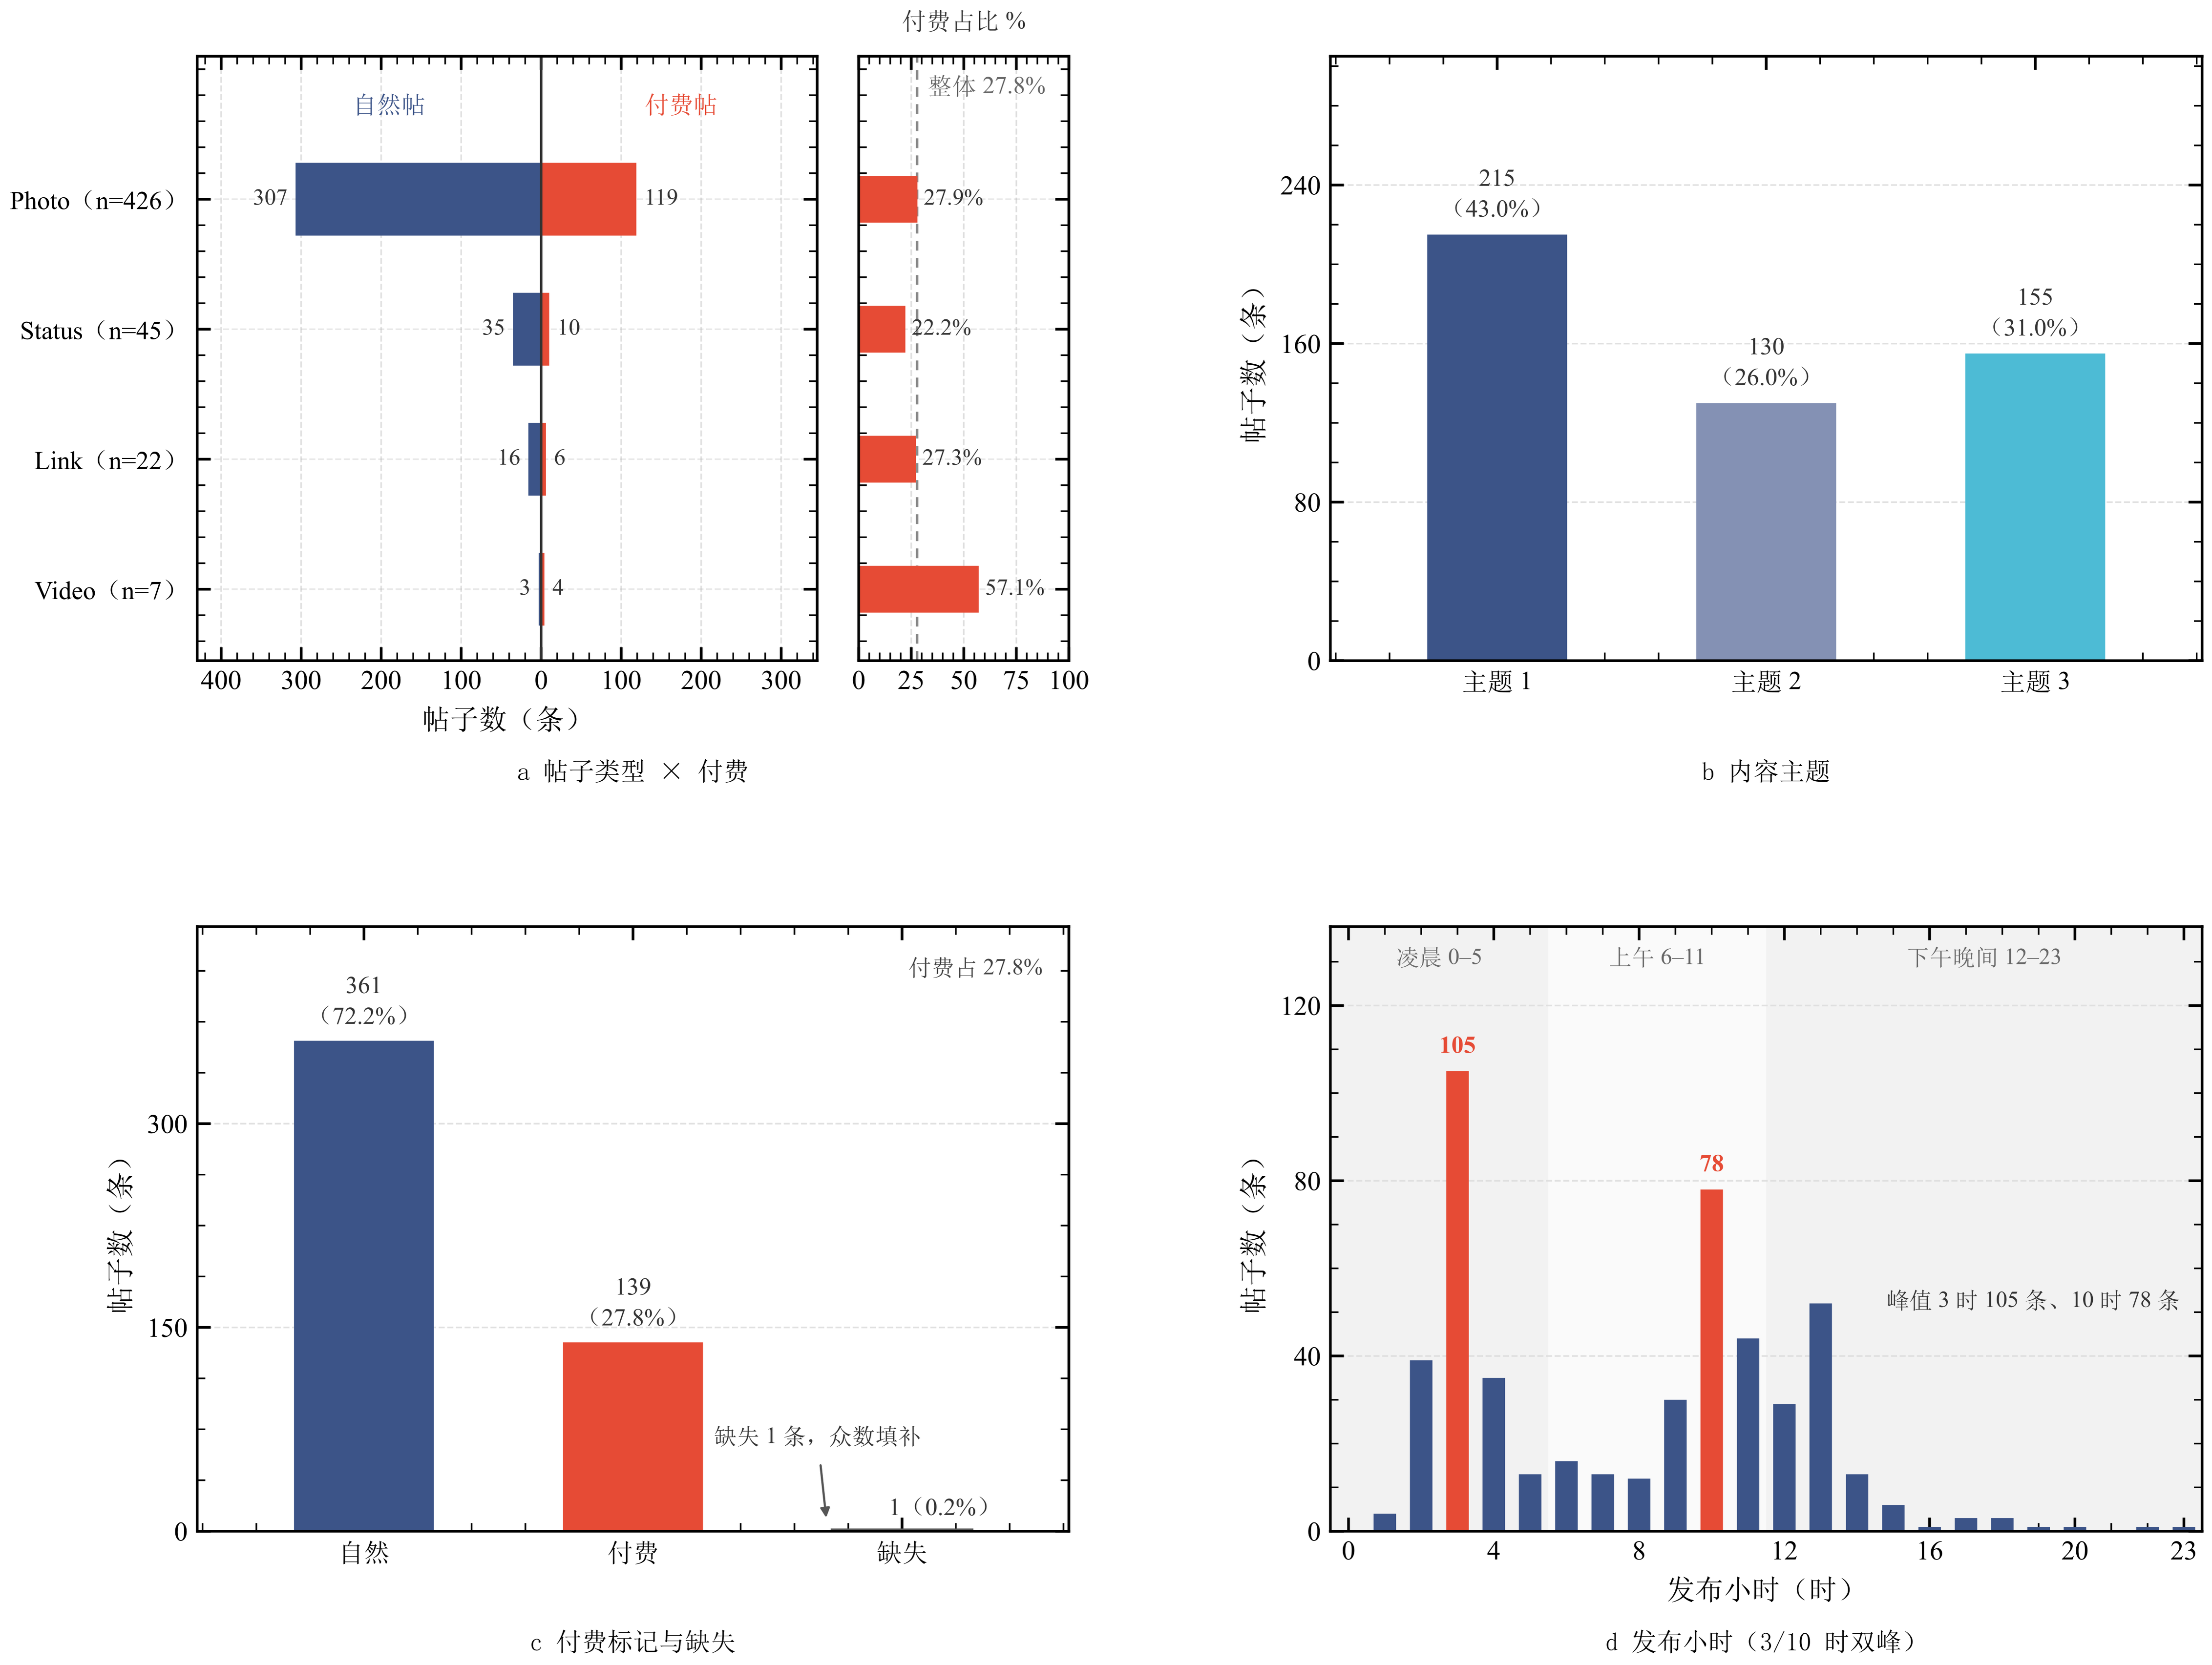
\includegraphics[width=0.62\textwidth]{../求解/问题二/结果/图4_类别结构与缺失.png}
  \caption{类别结构与缺失分布：类型、主题、付费标记与发布小时}
  \label{fig:cat}
\end{figure}

变换效果见表\ref{tab:transform}与图\ref{fig:trans}。$\log(1+Y_1)$ 把偏度从 8.33 压到 0.73、峰度从 93.05 压到 0.82，直方图接近对称，Q--Q 图主体贴合参考线；原始尺度下 Q--Q 图两端明显偏离，上尾尤其上翘。两端仍略有偏离，Jarque--Bera 检验 $p<0.001$，说明变换后仍非严格正态，这一点在残差诊断与稳健标准误的选择中被保留处理，而不是通过进一步变换掩盖。

{\small
\begin{longtable}{>{\centering\arraybackslash}p{0.080\textwidth}>{\centering\arraybackslash}p{0.140\textwidth}>{\centering\arraybackslash}p{0.140\textwidth}>{\centering\arraybackslash}p{0.140\textwidth}>{\centering\arraybackslash}p{0.140\textwidth}>{\centering\arraybackslash}p{0.140\textwidth}>{\centering\arraybackslash}p{0.160\textwidth}}
  \caption{变换前后的分布特征}
  \label{tab:transform} \\
  \toprule
  变量 & 偏度（前） & 偏度（后） & 峰度（前） & 峰度（后） & 最小值 & 最大值 \\
  \midrule
  \endfirsthead
  \caption{变换前后的分布特征（续）} \\
  \toprule
  变量 & 偏度（前） & 偏度（后） & 峰度（前） & 峰度（后） & 最小值 & 最大值 \\
  \midrule
  \endhead
  \bottomrule
  \endfoot
  Y1 & 8.3259 & 0.7341 & 93.0526 & 0.8209 & 570 & 1,110,282 \\
  X1 & -0.9795 & -1.1541 & -0.2759 & 0.1845 & 81,370 & 139,441 \\
\end{longtable}
}


\begin{figure}[htbp]
  \centering
  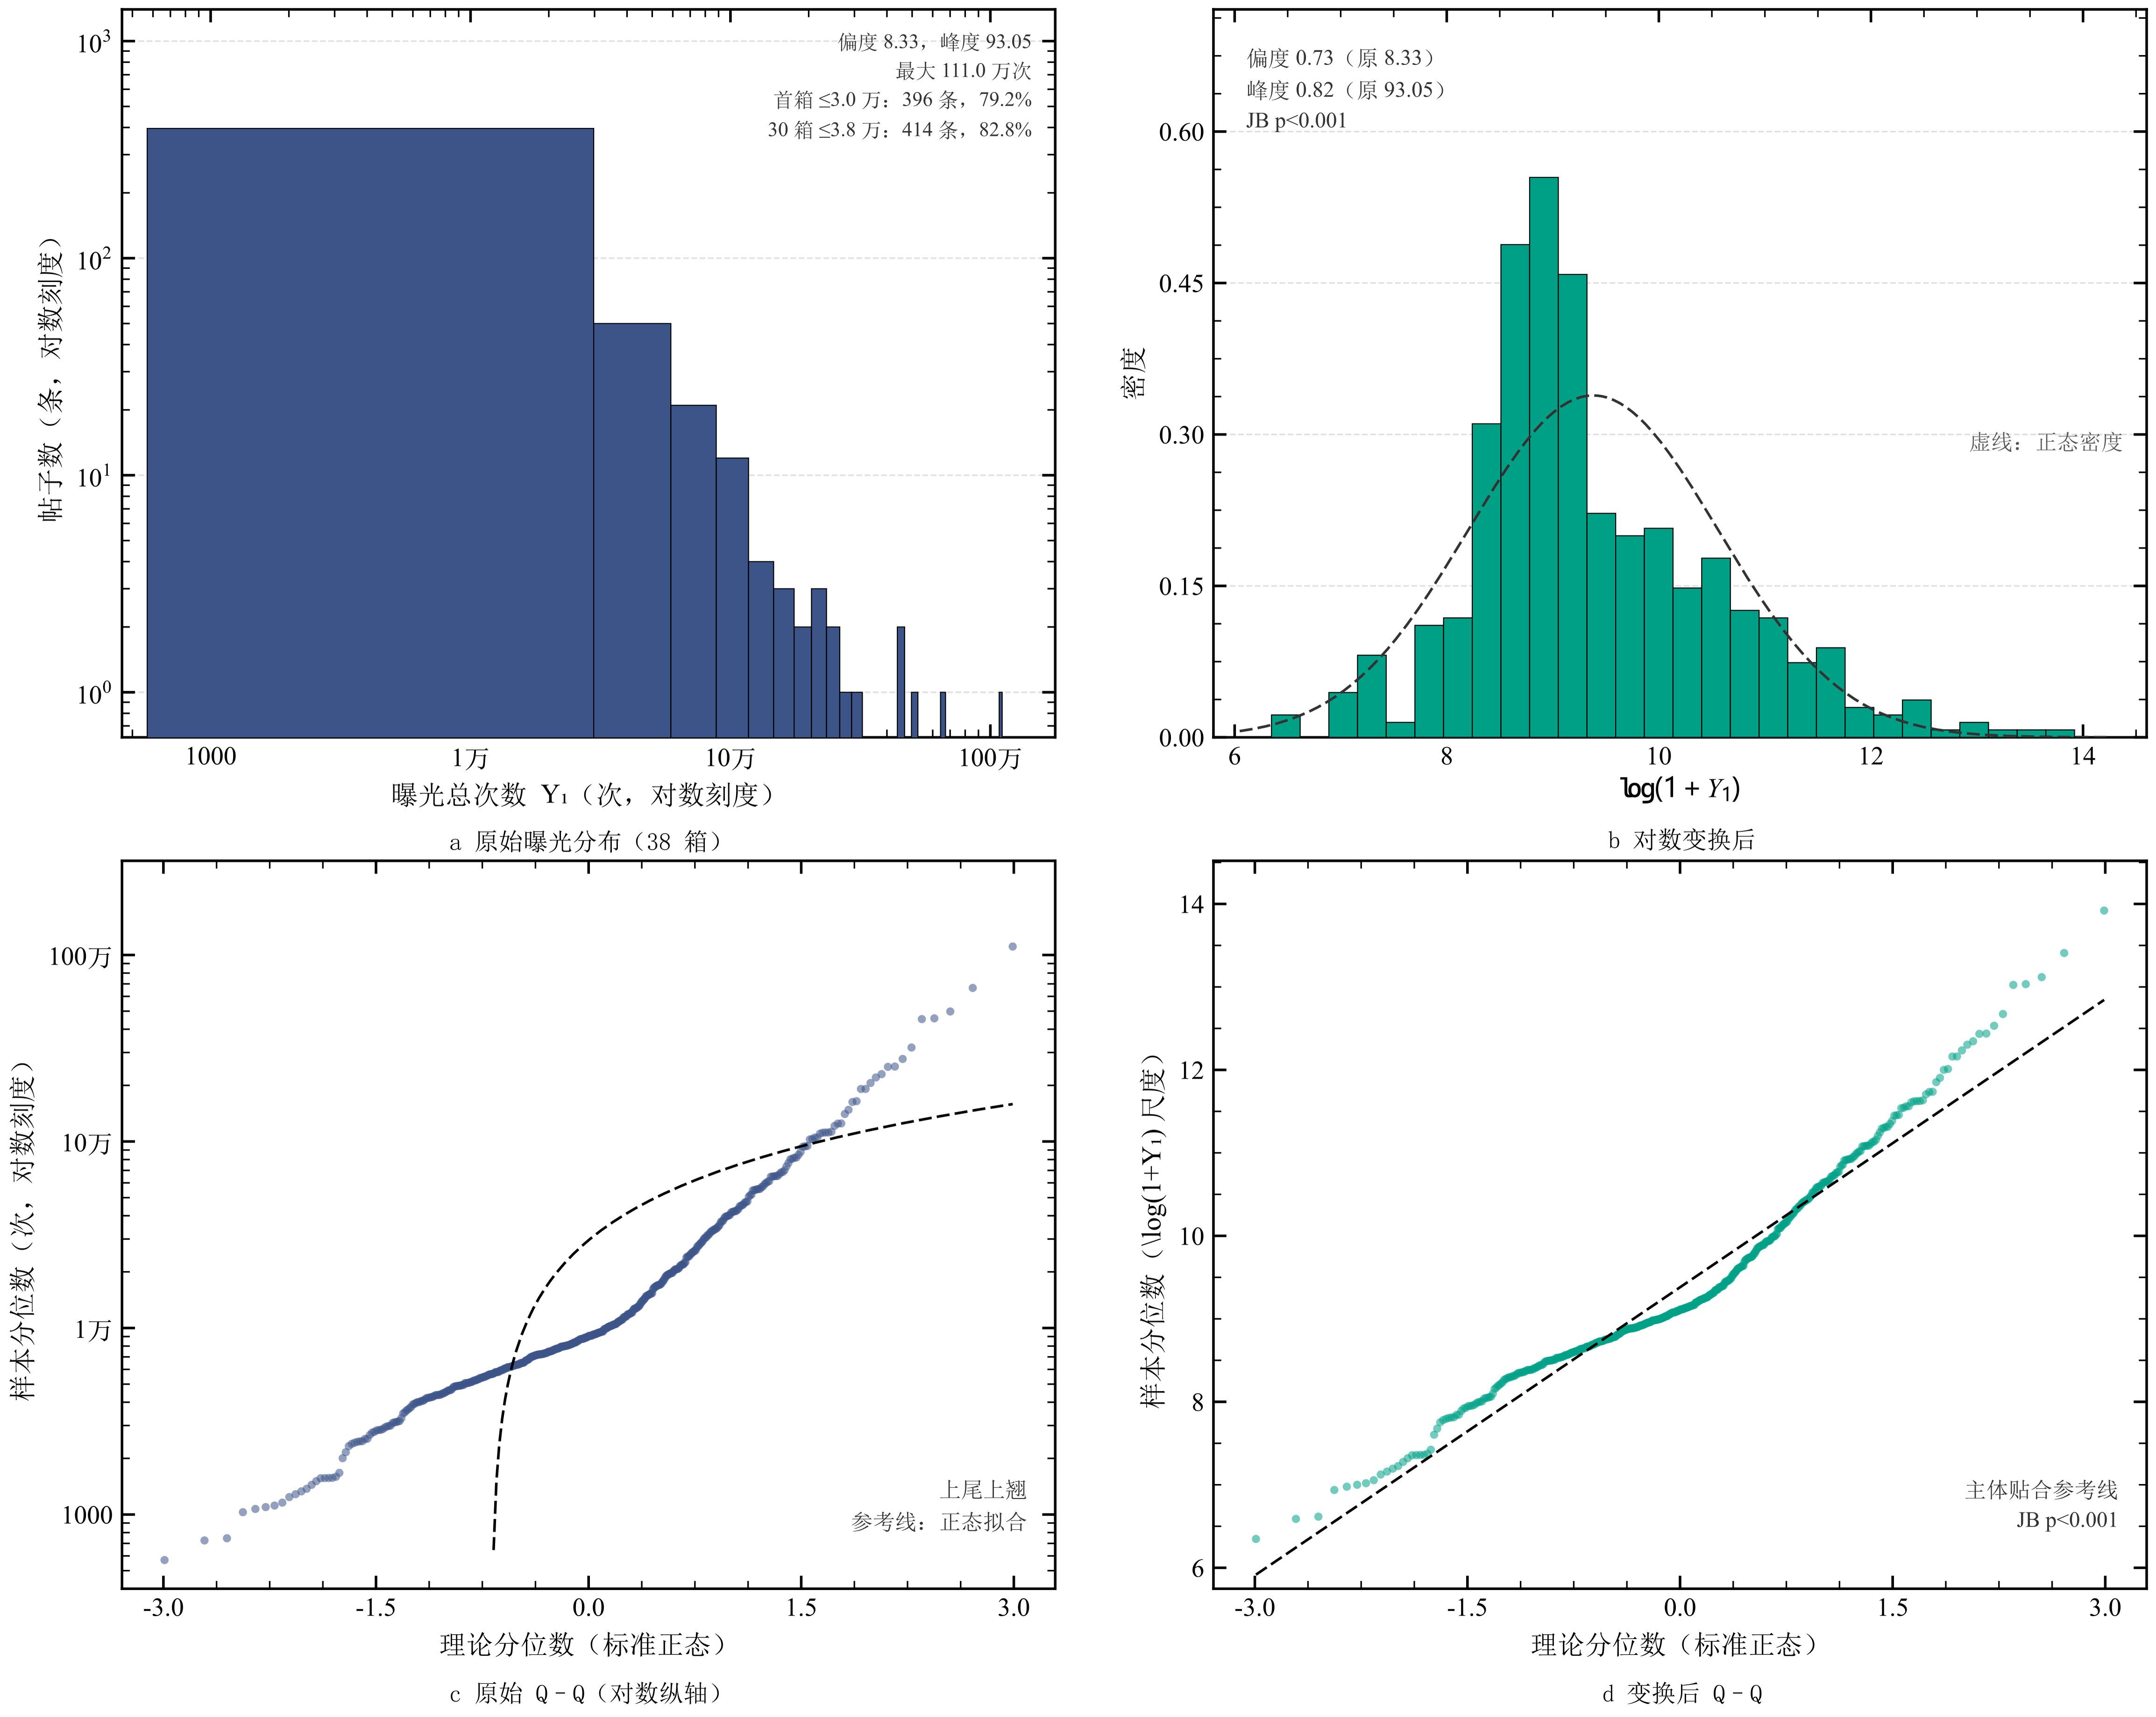
\includegraphics[width=0.60\textwidth]{../求解/问题二/结果/图5_变换前后分布.png}
  \caption{变换前后的分布与 Q--Q 图}
  \label{fig:trans}
\end{figure}

\subsection{共线诊断与识别策略}

粉丝规模与发布月份几乎同步：Pearson 相关 0.941、Spearman 相关 0.996；以月份哑变量对 $\log X_1$ 做辅助回归，$R^2=0.9917$，月内标准差仅 0.0130，月内方差占比 0.83\%（表\ref{tab:collinear}）。三项判据同时满足，说明两者属于同一变异维度，同时进入回归会使粉丝规模系数只由极少量月内变异驱动。图\ref{fig:collinear}把这个结构画出来：按月排列的散点几乎落在同一条单调上升曲线上，月均值折线与之重合，下挂小图显示每条帖子相对当月均值的偏差绝大多数落在 $\pm1{,}800$ 次以内，中位绝对偏差仅 582 次。

{\small
\begin{longtable}{>{\centering\arraybackslash}p{0.340\textwidth}>{\centering\arraybackslash}p{0.200\textwidth}>{\centering\arraybackslash}p{0.400\textwidth}}
  \caption{样本结构与共线判别指标}
  \label{tab:collinear} \\
  \toprule
  指标 & 数值 & 说明 \\
  \midrule
  \endfirsthead
  \caption{样本结构与共线判别指标（续）} \\
  \toprule
  指标 & 数值 & 说明 \\
  \midrule
  \endhead
  \bottomrule
  \endfoot
  样本量 & 500.0 & 500 条帖子 \\
  变量数 & 8 & 7 个输入 + 1 个输出 \\
  完全重复行 & 0 & 按 8 个原始变量判定 \\
  X7 缺失数 & 1 & 仅第 499 行缺失，占 0.2\% \\
  Y1 偏度（原始） & 8.3259 & 右偏严重，需 log1p \\
  Y1 峰度（原始） & 93.0526 & 超额峰度 \\
  Y1 最大值/中位数 & 122.7 & 极端重尾 \\
  log1p(Y1) 偏度 & 0.7341 & 变换后接近对称 \\
  log1p(Y1) 峰度 & 0.8209 & 变换后峰度显著下降 \\
  log(X1) 偏度 & -1.1541 & 左偏（粉丝数持续增长） \\
  Pearson r(X1, X4) & 0.9412 & 粉丝规模与月份的线性相关 \\
  Spearman ρ(X1, X4) & 0.9960 & 单调相关接近 1 \\
  R²(logX1 ~ 月份哑变量) & 0.9917 & 99.2\% 的粉丝规模变异在月间 \\
  log(X1) 总标准差 & 0.1435 & 跨全部帖子 \\
  log(X1) 月内标准差 & 0.0130 & 仅 1.3\%，月内几乎不变 \\
  月内方差占比 & 0.0083 & 1 - R² \\
  X1 唯一值数 & 90 & 90 个不同取值，重复多 \\
  月内 X1 唯一值中位数 & 6.5 & 每月仅约 6–7 个不同粉丝数 \\
  X1 最大值/最小值 & 1.7137 & 量级跨度有限 \\
\end{longtable}
}


\begin{figure}[htbp]
  \centering
  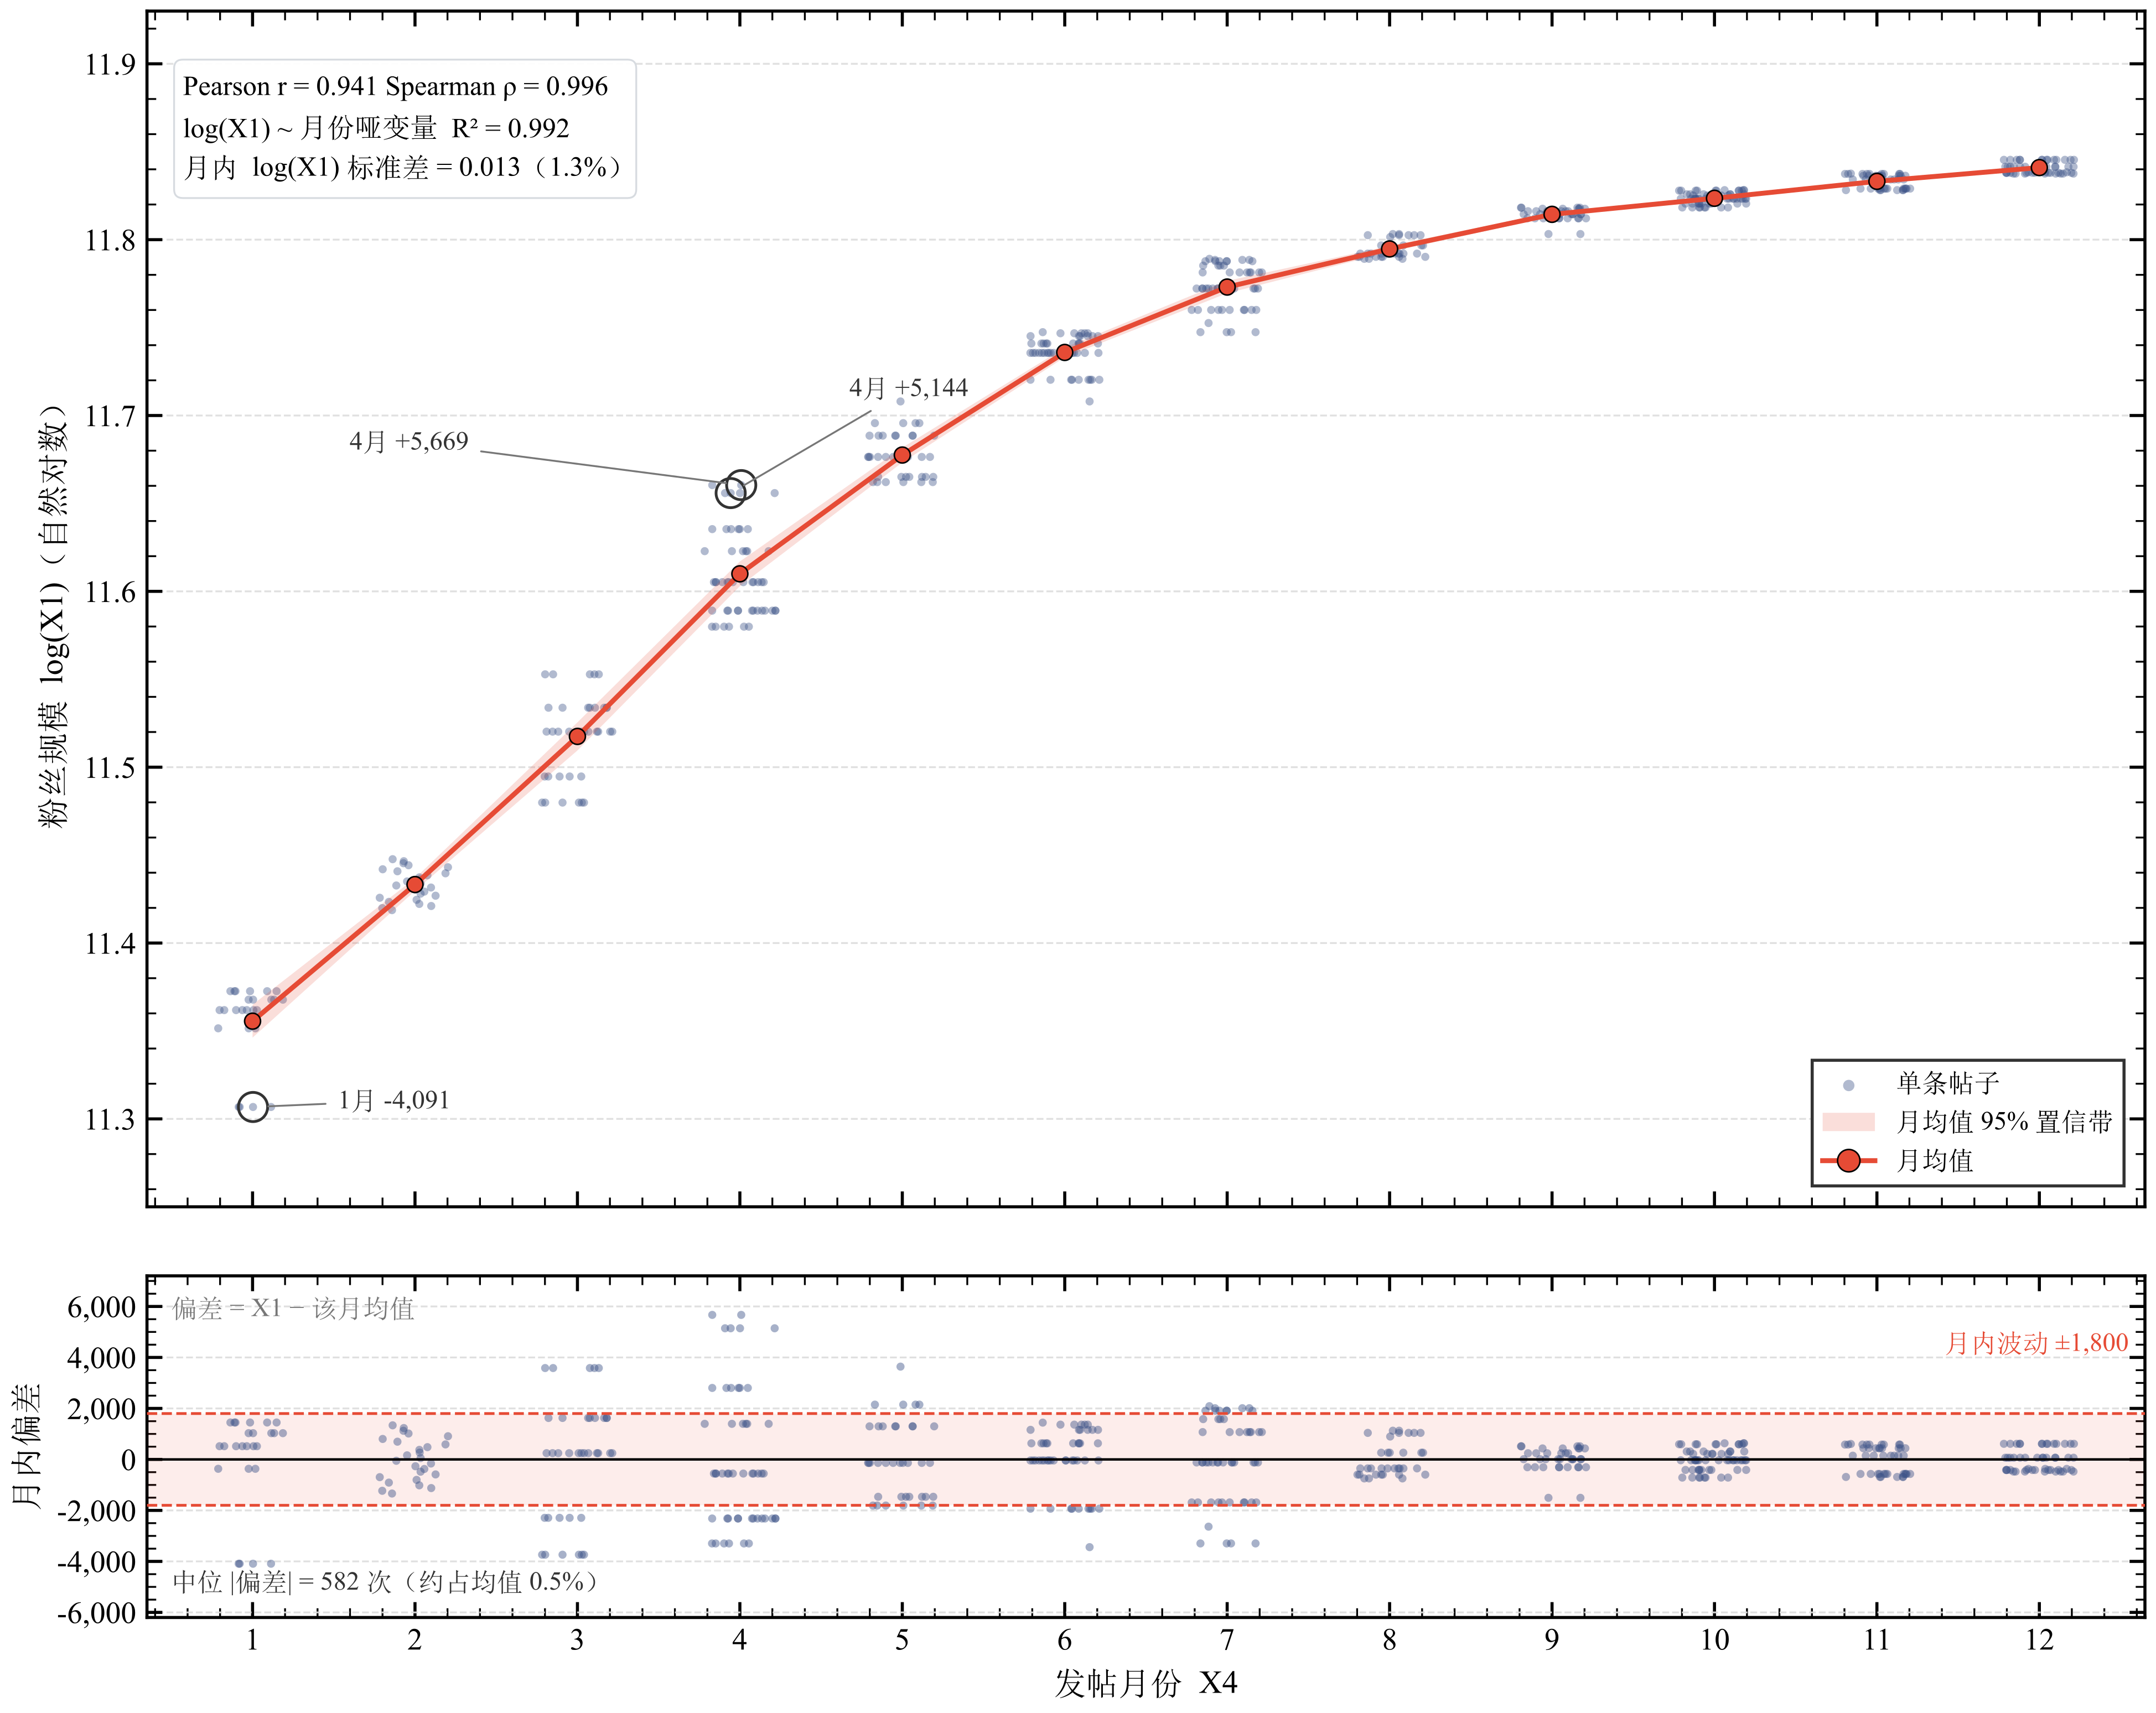
\includegraphics[width=0.63\textwidth]{../求解/问题一/结果/图2_粉丝规模与月份共线.png}
  \caption{粉丝规模与发布月份的共线结构：月度阶梯与月内偏差}
  \label{fig:collinear}
\end{figure}

据此确定识别策略：保留月份固定效应吸收规模趋势与季节波动，把粉丝规模留作稳健性对照（模型 M3、M4），而不强行解释其系数。这一处理在共线诊断上的直接效果是最大方差膨胀因子由 143.0 降至 3.23（第 6.3 节），代价是放弃了对“粉丝规模弹性”的因果解释——在单品牌、单期抓取的数据上，这个参数本身无法被识别。
